% www.overleaf.com

%cuidado ao mexer no arquivo configuracoes
%nao tente compilar de dentro dele, não irá funcionar
%caso faça isso, volte para este arquivo e tente novamente

\documentclass[
    article,
	% -- opções da classe memoir --
	12pt,				% 
	openright,			% capítulos começam em pág ímpar (insere página vazia caso preciso)
	oneside,
	%twoside,			% para impressão em verso e anverso. Oposto a oneside
	a4paper,			% tamanho do papel. 
	% -- opções da classe abntex2 --
	%chapter=TITLE,		% títulos de capítulos convertidos em letras maiúsculas
	section=TITLE,		% títulos de seções convertidos em letras maiúsculas
	subsection=TITLE,	% títulos de subseções convertidos em letras maiúsculas
	%subsubsection=TITLE,% títulos de subsubseções convertidos em letras maiúsculas
	% -- opções do pacote babel --
	english,			% idioma adicional para hifenização
	french,				% idioma adicional para hifenização
	spanish,			% idioma adicional para hifenização
	brazil,				% o último idioma é o principal do documento
	]{abntex2}
	

%atualizacao em 31-10-2022
\usepackage{abntex2/IFRN}

\usepackage{tgtermes}
\usepackage{fancyhdr}
\pagestyle{fancy}
\pagestyle{fancyplain}
\fancyhf{}
\lhead{}
\rhead{\thepage}
\rfoot{}
\renewcommand{\headrulewidth}{0pt}
% ---
% PACOTES
% ---

% ---
% Pacotes fundamentais 
% ---
\usepackage{lmodern}			% Usa a fonte Latin Modern
\usepackage[T1]{fontenc}		% Selecao de codigos de fonte.
\usepackage[utf8]{inputenc}		% Codificacao do documento (conversão automática dos acentos)
\usepackage{indentfirst}		% Indenta o primeiro parágrafo de cada seção.
\usepackage{color}				% Controle das cores
\usepackage{graphicx}			% Inclusão de gráficos
\usepackage{microtype} 			% para melhorias de justificação
\usepackage{float}
% ---
\usepackage{pdfpages}
\usepackage{caption}
\usepackage{subcaption}
%\usepackage[export]{adjustbox}
\usepackage{graphbox,graphicx}


% ---
% Pacotes adicionais, usados no anexo do modelo de folha de identificação
% ---
\usepackage{multicol}
\usepackage{multirow}
% ---
\usepackage[font=footnotesize]{caption}%textfont=bf,labelfont=bf,
\usepackage[table,xcdraw]{xcolor}


% ---
% Pacotes adicionais, usados apenas no âmbito do Modelo Canônico do abnteX2
% ---
\usepackage{lipsum}				% para geração de dummy text
% ---
\usepackage{titlesec}
\usepackage[left=3cm,top=3cm,right=2cm,bottom=2cm]{geometry}



% ---
% Pacotes de citações
% ---
\usepackage[brazilian,hyperpageref]{backref} % Paginas com as citações na bibl
\usepackage[alf,
            %versalete,
            abnt-emphasize = bf, % destaca o titulo em negrito;
            %abnt-etal-list = 3, % trabalhos com mais de 3 autores recebem et al.,;
            %abnt-etal-text = it, % escreve o et al., em italico;
            %abnt-and-type = &, % usa o carater '&' no lugar de 'e' para mais de um autor;
            %abnt-last-names = abnt, % trata sobrenomes 'estritamente' conforme a ABNT; e
            %abnt-repeated-author-omit = yes % autores com + de uma entrada recebem '____.'
]{abntex2cite}
% --- 
% CONFIGURAÇÕES DE PACOTES
% --- 



% ---
% Configurações do pacote backref
% Usado sem a opção hyperpageref de backref
\renewcommand{\backrefpagesname}{Citado na(s) página(s):~}
% Texto padrão antes do número das páginas
\renewcommand{\backref}{}
% Define os textos da citação
\renewcommand*{\backrefalt}[4]{
	\ifcase #1 %
		Nenhuma citação no texto.%
	\or
		Citado na página #2.%
	\else
		Citado #1 vezes nas páginas #2.%
	\fi}%
% ---




% ---
% Configurações de aparência do PDF final

% alterando o aspecto da cor azul
\definecolor{blue}{RGB}{41,5,195}

% informações do PDF
\makeatletter
\hypersetup{
     	%pagebackref=true,
		pdftitle={\@title}, 
		pdfauthor={\@author},
    	pdfsubject={\imprimirpreambulo},
	    pdfcreator={LaTeX with abnTeX2},
		pdfkeywords={abnt}{latex}{abntex}{abntex2}{relatório técnico}, 
		colorlinks=true,       		% false: boxed links; true: colored links
    	linkcolor=black,          	% color of internal links
    	citecolor=black,        		% color of links to bibliography
    	filecolor=magenta,      		% color of file links
		urlcolor=blue,
		bookmarksdepth=4
}
\makeatother
% --- 

% --- 
% Espaçamentos entre linhas e parágrafos 
% --- 

% O tamanho do parágrafo é dado por:
\setlength{\parindent}{1.3cm}

% Controle do espaçamento entre um parágrafo e outro:
\setlength{\parskip}{0.2cm}  % tente também \onelineskip


%atualizacao em 31-03-2021

\renewcommand{\imprimircapa}{%
\begin{capa}%
    \center
        \centering \nomeInstituicao 
        
        \vspace*{3cm}
        
        {\ABNTEXchapterfont\normalsize\imprimirautor} 
        
        \vspace*{4cm}
        
        {\ABNTEXchapterfont\bfseries\normalsize\imprimirtitulo} 
        \vspace*{\fill}
        
        {\normalsize\imprimirlocal} 
            \par
        {\normalsize\imprimirdata}
        
    \vspace*{1cm}
    
\end{capa}
}



\renewcommand{\imprimirfolhaderosto}{%
\begin{folhadeaprovacao}%
    \center
        
        {\ABNTEXchapterfont\normalsize\imprimirautor} 
        
        \vspace*{4cm}
        
        {\ABNTEXchapterfont\bfseries\normalsize\imprimirtitulo} 
        \vspace*{2cm}
        
        \hspace{.45\textwidth}
        \begin{minipage}{.5\textwidth}
            \singlespacing
            \imprimirpreambulo \\
            \\
            Orientador: \imprimirorientador
        \end{minipage}%
        
        \vspace*{\fill}
        
        {\normalsize\imprimirlocal} 
            \par
        {\normalsize\imprimirdata}
        
    \vspace*{1cm}
    
    \newpage
    
\end{folhadeaprovacao}
}

%atualizacao em 31-03-2021





%atualização em 31/10/2022
\usepackage{listings}

% ----------------------------------------------------------
% PERSONALIZAÇÃO DE CORES
% ----------------------------------------------------------
\definecolor{cinza}{HTML}{FCF8F8}
\definecolor{blue}{RGB}{41,5,195}
\definecolor{gray}{rgb}{.4,.4,.4}
\definecolor{gray}{rgb}{.4,.4,.4}
\definecolor{pblue}{rgb}{0.13,0.13,1}
\definecolor{pgreen}{rgb}{0,0.5,0}
\definecolor{pred}{rgb}{0.9,0,0}
\definecolor{pgrey}{rgb}{0.46,0.45,0.48}
\definecolor{lightgray}{rgb}{0.95, 0.95, 0.96}
\definecolor{whitesmoke}{rgb}{0.96, 0.96, 0.96}
\definecolor{javared}{rgb}{0.6,0,0} % for strings
\definecolor{javagreen}{rgb}{0.25,0.5,0.35} % comments
\definecolor{javapurple}{rgb}{0.5,0,0.35} % keywords
\definecolor{javadocblue}{rgb}{0.25,0.35,0.75} % javadoc
\definecolor{meucinza}{rgb}{0.5, 0.5, 0.5}
%\definecolor{lightgray}{gray}{0.9}

% define formato e estilo dos elementos do tipo Codigo Fonte
\lstset{language=PHP,
basicstyle=\ttfamily\scriptsize,
%basicstyle=\ttfamily,
keywordstyle=\color{javapurple}\bfseries,
stringstyle=\color{pblue},
commentstyle=\color{javagreen},
morecomment=[s][\color{javadocblue}]{/**}{*/},
morecomment=[s][\color{gray}]{@}{\ },
numbers=left,
numberstyle=\tiny\color{black},
backgroundcolor=\color{cinza},
stepnumber=2,
numbersep=8pt,
xleftmargin=14pt,
tabsize=4,
showspaces=false,
showstringspaces=false,
breaklines=true,}

%%%%%%%%%%%%%%%%%%%%%%%%%%%%%%%%%%



\newenvironment{ficha}{\textbf{Ficha catalográfica}}

\providecommand{\imprimirDataApresentacao}{}
\newcommand{\dataApresentacao}[1]{\renewcommand{\imprimirDataApresentacao}{#1}}

\providecommand{\imprimirPrimeiroMembroBanca}{}
\providecommand{\imprimirInstituicaoPrimeiroMembroBanca}{}
\newcommand{\primeiroMembroBanca}[2]{
    \renewcommand{\imprimirPrimeiroMembroBanca}{#1}
    \renewcommand{\imprimirInstituicaoPrimeiroMembroBanca}{#2}
}


\providecommand{\imprimirSegundoMembroBanca}{}
\providecommand{\imprimirInstituicaoSegundoMembroBanca}{}
\newcommand{\segundoMembroBanca}[2]{
    \renewcommand{\imprimirSegundoMembroBanca}{#1}
    \renewcommand{\imprimirInstituicaoSegundoMembroBanca}{#2}
}



\newcommand{\folhaaprovacao}{
%
\begin{folhadeaprovacao}

  \begin{center}
    {\ABNTEXchapterfont\large\imprimirautor}

    \vspace*{\fill}\vspace*{\fill}
    \begin{center}
      \ABNTEXchapterfont\bfseries\normalsize\imprimirtitulo
    \end{center}
    \vspace*{2cm}
    
    \hspace{.45\textwidth}
    \begin{minipage}{.5\textwidth}
        \imprimirpreambulo
    \end{minipage}%
    \vspace*{\fill}
   \end{center}
        
   Trabalho aprovado. \imprimirlocal, \imprimirDataApresentacao.
   \newline
   \newline
   \centering BANCA EXAMINADORA


   %sempre manter o título acadêmico dos professores
   \assinatura{\textbf{\imprimirorientador} \\ Orientador - IFRN} 
   \assinatura{\textbf{\imprimirPrimeiroMembroBanca} \\ \imprimirInstituicaoPrimeiroMembroBanca}
   \assinatura{\textbf{\imprimirSegundoMembroBanca} \\ \imprimirInstituicaoSegundoMembroBanca}

    \newpage
\end{folhadeaprovacao}
}


%%%%%%%%%%%%%%%%%%%%%%%%%%%%%%%%%%%%%%%%
\newcommand{\espacofichacatalografica}{
\begin{ficha}
    \centering Aqui entrará a ficha catalográfica
    \newpage
\end{ficha}
}



% após a defesa a ficha catalográfica é gerada
% então o trecho acima deve ser comentado
% a linha abaixo deve ser descomentada
%\includepdf[pages=-]{ficha-catalografica.pdf}

% ---
% compila o indice
% ---
\makeindex
% ---



% ---
% Informações de dados para CAPA e FOLHA DE ROSTO
% ---
\titulo{Título: Subtítulo}
\autor{Fulanilson Pereira da Silva}
\local{Nova Cruz/RN}
%Sempre adicione a titulação do professor
%Ele pode ficar bem zangado se for esquecido
\orientador{Profa. Dra. Ciclanilsa Pereira}
\primeiroMembroBanca{Prof. Me. Percivaldo Abrupto}{Examinador interno - IFRN}
\segundoMembroBanca{Prof. Dr. Agrônio Morolov}{Examinador interno - IFRN}
\dataApresentacao{28 de Agosto de 2022}
\data{2021}
\newcommand{\nomeInstituicao}{INSTITUTO FEDERAL DE EDUCAÇÃO, CIÊNCIA E TECNOLOGIA DO RIO GRANDE DO NORTE}
\instituicao{%
  \nomeInstituicao -- IFRN
  \par
  Técnico Integrado em Informática}
\tipotrabalho{Relatório técnico}
% O preambulo deve conter o tipo do trabalho, o objetivo, 
% o nome da instituição e a área de concentração 
\preambulo{Trabalho de Conclusão de Curso apresentado ao
Curso Superior de Tecnologia em Análise e
Desenvolvimento de Sistemas do Instituto Federal de
Educação, Ciência e Tecnologia do Rio Grande do
Norte, em cumprimento às exigências legais como
requisito parcial à obtenção do título de Tecnólogo
em Análise e Desenvolvimento de Sistemas.}
% ---



% ----
% Início do documento
% ----
\begin{document}

% Retira espaço extra obsoleto entre as frases.
\frenchspacing 

%esse include precisava ficar depois do \begin{document}
%atualizacao em 31-10-2022 (Todo o arquivo)
%esse includes precisavam ficar depois do \begin{document}


\titleformat{\section}{\normalfont\bfseries\uppercase}{\thesection}{1em}{}
\titlespacing*{\section}{0cm}{0.60cm}{0.70cm}
\titleformat{\subsection}{\normalfont\uppercase}{\thesubsection}{1em}{}
\titlespacing*{\subsection}{0cm}{0.60cm}{0.70cm}
\titleformat{\subsubsection}{\normalfont\bfseries}{\thesubsubsection}{1em}{}
\titlespacing*{\subsubsection}{0cm}{0.60cm}{0.70cm}

\titleformat{\subsubsubsection}{\normalfont}{\thesubsubsubsection}{1em}{}
\titlespacing*{\subsubsubsection}{0cm}{0.60cm}{0.70cm}


%secao quaternaria
\renewcommand*{\thesubparagraph}{\alph{subparagraph}}
\titleformat{\paragraph}
{\normalfont\normalsize}{\theparagraph}{1em}{}
\titlespacing*{\paragraph}{0cm}{0.60cm}{0.70cm}
\renewcommand{\subsubsubsection}{\paragraph}
%%%%%%%%%%%%%%%%%%



\renewcommand{\agradecimentosname}{\textbf{AGRADECIMENTOS}}
\renewcommand{\resumoname}{\textbf{RESUMO}}
\renewcommand{\listadesiglasname}{\textbf{LISTA DE SIGLAS}}
\renewcommand{\listadesimbolosname}{\textbf{LISTA DE SÍMBOLOS}}
\renewcommand{\listfigurename}{\textbf{LISTA DE ILUSTRAES}}
\renewcommand{\listtablename}{\textbf{LISTA DE TABELAS}}
\renewcommand{\listfigurename}{\textbf{LISTA DE ILUSTRAÇÕES}}
%\renewcommand{\listquadrosname}{\textbf{LISTA DE QUADROS}}
\renewcommand{\contentsname}{\textbf{SUMÁRIO}}


% ----------------------------------------------------------
% ELEMENTOS PRÉ-TEXTUAIS
% ----------------------------------------------------------
% \pretextual

% ---
% Capa
% ---
\imprimircapa
% ---


% ---
% Folha de rosto
% (o * indica que haverá a ficha bibliográfica)
% ---
\imprimirfolhaderosto
% ---


\espacofichacatalografica

\folhaaprovacao

% ---
% ---
% Agradecimentos
% ---
\begin{agradecimentos}
A todos os professores do Instituto Federal de Educação, Ciência Tecnologia do Rio Grande do Norte (IFRN) que colaboraram e construíram bases sólidas no meu desenvolvimento e aprendizagem para o crescimento profissional.
Seus nomes são inesquecíveis e por isso, dedico-lhes minha profunda admiração e respeito.

A todos aqueles que acreditaram na realização deste trabalho e deram-me forças e estímulo para dar prosseguimento a esta pesquisa e obter sucesso. Em especial, o meu orientador, Professor Fulano Aquino Rêgo, e aos meus colegas de turma. 

A Deus criador dos céus e da terra, o que me deu a vida.
\newpage
\end{agradecimentos}
% ---

% ---
% RESUMO
% ---

% resumo na língua vernácula (obrigatório)
\setlength{\absparsep}{18pt} % ajusta o espaçamento dos parágrafos do resumo
\begin{resumo}
 Elemento obrigatório, constituído de uma sequência de frases concisas e não
de uma simples enumeração de tópicos. Segundo a ABNT, o resumo deve ressaltar o objetivo, o método, os resultados e as conclusões do documento. Deve ser constituído de um parágrafo único e conter 150 a 500 palavras. A primeira frase significativa relacionada ao tema. Deve conter: Objetivo, metodologia, resultados e conclusões nessa ordem. Usar verbo na voz ativa e na terceira pessoa do singular. Evitar símbolos, contrações, fórmulas, equações, e diagramas. Inclui palavras-chave, separadas entre si por ponto e finalizadas também por ponto.
 
 \noindent
 %Palavras chave em ordem de importância ou alfabética, separadas por ;
 \textbf{Palavras-chave}: elemento obrigatório; parágrafo único; terceira pessoa do singular.
 \newpage
\end{resumo}
% ---


% ---
% ABSTRACT
% ---

% resumo na língua vernácula (obrigatório)
\setlength{\absparsep}{18pt} % ajusta o espaçamento dos parágrafos do resumo
\begin{resumo}[\textbf{ABSTRACT}]
\begin{otherlanguage*}{english}


 Mandatory element, consisting of a sequence of concise sentences and not
of a simple enumeration of topics. According to ABNT, the abstract should emphasize the objective, method, results and conclusions of the document. It must consist of a single paragraph and contain 150 to 500 words. The first meaningful sentence related to the topic. It must contain: Objective, methodology, results and conclusions in that order. Use verb in the active voice and in the third person singular. Avoid symbols, contractions, formulas, equations, and diagrams. It includes keywords, separated from each other by a period and also ending with a period.


\end{otherlanguage*}
 
 \noindent
 \textbf{Key words}: mandatory element; single paragraph; third person singular.
 \newpage
\end{resumo}
% ---

\newpage

% ---
% inserir lista de ilustrações
% ---
\pdfbookmark[0]{\listfigurename}{lof}
\listoffigures*
\cleardoublepage
% ---


% ---
% LISTA DE CÓDIGOS FONTES
% ---

\pdfbookmark[0]{\lstlistingname}{lol} % caso não tenha códigos, comente esta linha 
\counterwithout{lstlisting}{chapter}
% Altera o nome padrão do rótulo usado no comando \autoref{}
\renewcommand{\lstlistingname}{Código Fonte}

% Altera o rótulo a ser usando no elemento pré-textual "Lista de código"
\renewcommand{\lstlistlistingname}{\textbf{LISTA DE CÓDIGOS}}
% Configura a ``Lista de Códigos'' conforme as regras da ABNT (para abnTeX2)
\begingroup\makeatletter
\let\newcounter\@gobble\let\setcounter\@gobbletwo
  \globaldefs\@ne \let\c@loldepth\@ne
  \newlistof{listings}{lol}{\lstlistlistingname}
  \newlistentry{lstlisting}{lol}{0}
\endgroup

\renewcommand{\cftlstlistingaftersnum}{\hfill--\hfil}

\let\oldlstlistoflistings\lstlistoflistings
{
\let\oldnumberline\numberline
\newcommand{\algnumberline}[1]{Código Fonte~#1~\enspace--~\enspace}
\renewcommand{\numberline}{\algnumberline}

\begin{KeepFromToc}
\lstlistoflistings
\end{KeepFromToc}
}
\cleardoublepage


%atualizacao em 31-10-2022
% ---
% LISTA DE QUADROS
% ---
\pdfbookmark[0]{\listofquadrosname}{loq} % caso não tenha quadros, comente esta linha 
\listofquadros* % caso não tenha quadros, comente esta linha 
\cleardoublepage



% ---
% inserir lista de tabelas
% ---
\pdfbookmark[0]{\listtablename}{lot}
\listoftables*
\cleardoublepage
% ---



% ---
% inserir lista de abreviaturas e siglas
% ---
\begin{siglas}
  \item[Fig.] Area of the $i^{th}$ component
  \item[456] Isto é um número
  \item[123] Isto é outro número
  \item[lauro cesar] este é o meu nome
\end{siglas}
% ---

% ---
% inserir lista de símbolos
% ---
\begin{simbolos}
  \item[$\Gamma$] Letra grega Gama
  \item[$\Lambda$] Lambda
  \item[$\zeta$] Letra grega minúscula zeta
  \item[$\in$] Pertence
\end{simbolos}
% ---

% ---
% inserir o sumario
% ---
\pdfbookmark[0]{\contentsname}{toc}
\tableofcontents*
\cleardoublepage
% ---


% ----------------------------------------------------------
% ELEMENTOS TEXTUAIS
% ----------------------------------------------------------
\textual

% ----------------------------------------------------------
% Introdução
% ----------------------------------------------------------
\secao{Introdução}

A introdução é a parte inicial do texto, onde devem constar a delimitação do assunto tratado, objetivos da pesquisa e outros elementos necessários para situar o tema do trabalho.

A Associação Brasileira de Normas Técnicas (ABNT) é um exemplo de nome cuja sigla é comumente utilizada, sempre que você usar uma sigla, a primeira vez que ela aparecer, deve vir precedida do seu nome por extenso. Nas próximas vezes em que aparecer no texto, basta utilizar a sigla.

O documento exemplifica a elaboração de relatórios técnicos e/ou científicos produzidos conforme a ABNT NBR 10719:2011 \emph{Informação e documentação - Relatório técnico e/ou científico - Apresentação}.


Ao final da introdução, \textbf{você deve explicar} o que o leitor irá encontrar nas próximas seções.

O presente trabalho é estruturado em cinco partes. Na primeira é apresentada a introdução, onde é proposta uma visão geral sobre o projeto. A segunda parte é a do \nameref{ref_teorico} que contém uma apresentação de conceitos relacionados ao desenvolvimento
do projeto. A terceira parte é a da \hyperref[sec:metodologia]{Metodologia}, em que é apresentado os métodos
utilizados para o desenvolvimento do projeto.

% ----------------------------------------------------------
% Capitulo com exemplos de comandos inseridos de arquivo externo 
% ----------------------------------------------------------
\subsecao{Justificativa}

Nesta etapa você deverá convencer o leitor sobre a importância do seu trabalho.

\subsubsecao{Objetivo}

Você deve definir um objetivo simples, preferencialmente que a solução do problema seja o objetivo e não a construção do sistema.
Ex:
O objetivo deste trabalho é solucionar o problema de superlotação na empresa X.

Uma vez analisados os problemas, chegou-se a conclusão de que o problema pode ser solucionado ou amenizado com um aplicativo Y que irá fazer Z coisas, assim diminuindo o problema de superlotação.

OBS: Defina um objetivo que você realmente poderá cumprir e que poderá ser verificado, por exemplo, ``O objetivo deste trabalho é melhorar o aprendizado da linguagem X'', ao final você vai conseguir provar que você melhorou o aprendizado? Você aplicará testes nos alunos para verificar isso? Se não, então é melhor escrever o objetivo de uma forma diferente, algo como, ``Propor uma nova forma ou uma nova ferramenta para... ''.

\subsubsubsecao{Objetivos específicos}

Aqui você irá listar alguns objetivos específicos, que seriam pontos que você precisa percorrer para chegar ao seu objetivo final. Obs, não listar objetivos muito óbvios como, ``Realizar levantamento bibliográfico'' e nem amarrar tanto  a solução do problema, ex: Se o problema for superlotação ele pode ser resolvido de várias formas, o aplicativo é apenas uma delas, então um objetivo ruim seria: "Construir o aplicativo Y"

Exemplos:

\begin{itemize}
\item Entender o funcionamento da empresa X
\item Elaborar uma solução, ou projeto
\item Construir o projeto
\item Implantar a solução
\end{itemize}



\subsubsecao{Referencial teórico}

\label{ref_teorico}

Aqui você deve abordar todos os aspectos teóricos nos quais o seu trabalho se embasou. Para isso você provavelmente irá precisar realizar várias citações.


Conforme a NBR 10520:2002, a citação é a menção de uma informação extraída de outra fonte. Pode ser direta ou indireta e deve ser composta pelo
sobrenome do autor, instituição responsável ou título, ano e paginação, conforme as especificidades apresentadas a seguir:

Citação direta é a transcrição textual de parte da obra do autor consultado. As citações diretas, no texto, de até três linhas, devem estar entre aspas duplas.


Ex.:


Segundo \citeonline[p. 15]{hair2009analise} ``Alguma frase dita pelo autor''.

``Alguma frase dita pelo autor'' \cite[p. 15]{hair2009analise}.

Citações diretas com mais de três linhas, devem ser destacadas com recuo de 4cm da margem esquerda, com letra tamanho 10, sem aspas;

Ex.:

\begin{citacao}
Entretanto, possuir informações, transmiti-las e acessá-las de forma rápida e direcionada, não significa, por si só, ter conhecimento sobre um determinado assunto. Conhecer requer algo mais, que é reunir as informações acessadas considerando-se um objetivo ou realidade, e, a partir destes, organizá-las de um modo lógico, que permita a produção de um novo conhecimento sobre o assunto que gerou o estudo. Em suma, conhecer exige a capacidade interpretativa do homem \cite[p. 22]{hair2009analise}.
\end{citacao}

Citação Indireta é a construção de um texto baseado na ideia de um autor consultado. As citações indiretas devem ser apresentadas pelo sobrenome do autor, instituição responsável ou título e ano:

Sobrenome do autor, no texto – Minúsculos.
Ex.: Segundo \citeonline[p. 20]{doneda2006privacidade}.

Sobrenome do autor, fora do texto, nos parênteses – Maiúsculos.
Ex.: \cite[p. 20]{paulino2006analise}.

Citação de páginas web, para fazer essas citações é preciso construir o código que vai para o bib, para isso é preciso descobrir o ano de publicação e autor. Muitas vezes o nome do autor vem na própria publicação, o nome do site só poderá ser usado se o nome do autor não constar na página. O ano de publicação também pode ser encontrado na página, porém é mais comum que não exista essa informação, então você pode procurar pelo ano em que o Google indexou a página. Basta fazer uma pesquisa no Google que encontre a página e utilizar junto o filtro de datas, com isso o Google irá mostrar a data de indexação junto com os resultados. Exemplo da citação online \cite{refABNTSite}.


Pode notar que tudo que é citado aparece automaticamente no final do documento em referências.

\subsubsubsecao{Tecnologias utilizadas}

Aqui você pode listar as tecnologias utilizadas, uma seção para cada uma. É importantíssimo destacar o motivo da escolha de cada tecnologia.


\secao{Metodologia}
\label{sec:metodologia}

Na metodologia você irá descrever todo o passo a passo que você realizou para construir o seu projeto.
Ex: Primeiramente foi necessário fazer um levantamento bibliográfico utilizando as bases de dados do Google \textit{Scholar} e a palavra-chave "COVID-19". Após este levantamento bibliográfico foram feitas reuniões com o cliente, a partir dos resultados das reuniões foram gerados gráficos.

Não esqueça de explicar detalhadamente como foi a metodologia de desenvolvimento, se foi Scrum, Xp, OpenUp, ou se não foi nenhuma delas e sim algo baseado em princípios ágeis, que é o mais comum.

É interessante construir algum tipo de cronograma.



\subsecao{Desenvolvimento}
\label{desenvolvimento}

Aqui você irá mostrar o seu trabalho.

\subsubsecao{Seção Terciária}
\label{outrasecao}

Pode ser dividido em subseções

\subsubsubsecao{Seção quaternária}

Ou subseções das subseções

Em seguida um exemplo de como fazer uma listagem de itens.

\noindent Descrever brevemente:
\begin{itemize}
\item A lei;
\item Objetivo;
\item Carga horária;
\item Jornada de trabalho.

\end{itemize}

Este parágrafo contém um exemplo de nota de rodapé\footnote{A nota de rodapé serve para explicar algum termo no rodapé da página, de forma que a leitura não é interrompida pela explicação}.

Toda figura ou tabela deve ser referenciada e EXPLICADA, dizendo ``A Figura X representa tal coisa, e isso funciona assim por causa disso e daquilo, lembrar de sempre escrever Figura com F maiúsculo''. Aqui também está o exemplo de como se deve usar as aspas. A Figura \ref{figura:qualquernome} é um exemplo de inclusão de imagem.

%normalmente o latex ira procurar o melhor lugar no documento para encaixar a imagem/tabela, mas isso pode atrapalhar a leitura
\begin{figure}[h]% o h faz com que ele procure um bom lugar para a imagem, mas isso pode bagunçar em alguns casos, use o H (maiúsculo) para forçar ela a ficar no local determinado
    \caption{Exemplo de imagem}
    \centering
    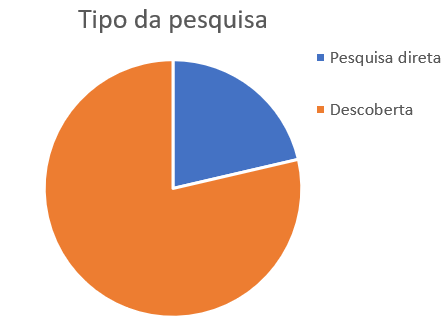
\includegraphics[width=5cm]{imagens/grafico.png}
    \label{figura:qualquernome}
    \fonteimagem{Fonte: Elaborado pelo autor}
\end{figure}


Exemplo com duas imagens a Figura \ref{fig:a} é a figura da esquerda e a Figura \ref{fig:b} é a figura da direita.

\begin{figure}[H]
     \centering
     \caption{Telas de Nova renovação}
     \begin{subfigure}[t]{0.40\textwidth}
         \centering
        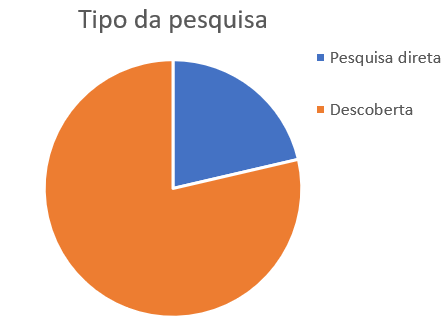
\includegraphics[width=\textwidth]{imagens/grafico.png}
         \caption{Selecionar paciente cadastrado}%
         \label{fig:a}
     \end{subfigure} %nao pode ter espaço aqui, aí fica uma ao lado da outra
     \begin{subfigure}[t]{0.40\textwidth}
         \centering
         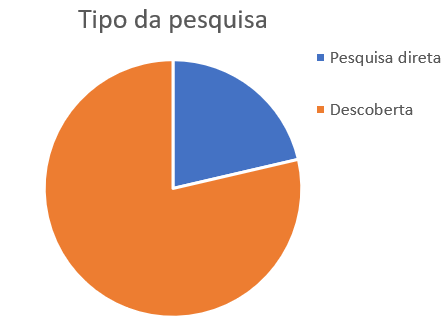
\includegraphics[width=\textwidth]{imagens/grafico.png}
         \caption{Formulário de nova renovação}%
         \label{fig:b}
     \end{subfigure}
     
    \fonteimagem{Fonte: Elaborado pelo autor}
    \label{fig:13}
\end{figure}

Dica: é comum o desenvolvimento de protótipos, quando assim for, coloque-os todos dentro de um apêndice e indique: os protótipos construídos estão disponíveis no Apêndice \ref{appendix:prototipos} deste documento. Os anexos são para documentos que você não produziu, mas que acha importante para o texto.

\newpage

Há uma diferença entre tabelas e quadros, tabelas não possuem linhas verticais, quadros possuem, no mais são muito semelhantes, inclusive a apresentação no texto. O Quadro \ref{quad:ex} é um exemplo. Sugiro o uso do site \url{https://www.tablesgenerator.com/} para gerar o código:



\begin{quadro}
\caption{Exemplo de quadro}
\label{quad:ex}
\centering
\begin{tabular}{|l|c|c|c|}
\hline
\multicolumn{1}{|c|}{} & \multicolumn{1}{l|}{\textbf{Qtd}} & \multicolumn{1}{l|}{\textbf{Valor R\$}} & \multicolumn{1}{l|}{\textbf{Tipo}} \\ \hline
\rowcolor[HTML]{FFCC67} 
\textbf{Produto A}     & 2                                 & 22                                      & C22                                \\ \hline
\textbf{Produto C}     & 3                                 & 33                                      & C88                                \\ \hline
\textbf{Produto D}     & 4                                 & 11                                      & c40                                \\ \hline
\end{tabular}
\fonteimagem{Fonte: Elaborado pelo autor}
\end{quadro}


A Tabela \ref{tab:ex} é um exemplo de tabela, não possui linhas verticais.



\begin{table}[h]% o h força a imagem/tabela a ficar neste local
\caption{Minha tabela}
\label{tab:ex}
\centering
\begin{tabular}{lccc}
\hline
\multicolumn{1}{c}{} & \multicolumn{1}{l}{\textbf{Qtd}} & \multicolumn{1}{l}{\textbf{Valor R\$}} & \multicolumn{1}{l}{\textbf{Tipo}} \\ \hline
\rowcolor[HTML]{FFCC67} 
\textbf{Produto A}     & 2                                 & 22                                      & C22                                \\ \hline
\textbf{Produto C}     & 3                                 & 33                                      & C88                                \\ \hline
\textbf{Produto D}     & 4                                 & 11                                      & c40                                \\ \hline
\end{tabular}
\fonteimagem{Fonte: Elaborado pelo autor}
\end{table}

Também é possível incluir fórmulas matemáticas, caso esteja com dificuldade para construir as equações, construa a equação em https://pt.symbolab.com/solver/equation-calculator, copie e cole aqui, obs, a equação deve estar entre \$equação\$ ou \$\$equação\$\$ (destacada). Outro detalhe é que não pode haver espaços entre o sinal \$ e a equação, exemplo:

$$x^n + y^n = z^n$$

Para incluir o sinal de porcentagem (\%) e outros sinais(\$ \# \^ \space \& \_ \{ \} \~ \space ) é necessário escapar o sinal com a barra invertida ($\backslash$).

O Código Fonte \ref{lst:exemplocodigo1} é um exemplo de como colocar código no documento.


%exemplo de código fonte, as configurações estão no arquivo packages.tex
\lstinputlisting[language=PHP, 
caption=Uma função em PHP
,label=lst:exemplocodigo1]{trechos_codigo/php.m}


\secao{Conclusão}

Por fim, a parte final do texto, na qual se apresentam conclusões correspondentes aos objetivos. Relembre se os objetivos foram concluídos, faça alguma discussão sobre os resultados e sugira trabalhos futuros.

OBS: NUNCA diga que não fez algo porque não deu tempo, se não daria tempo por que foi planejado? Se foi planejado e não deu tempo, você não administrou corretamente o projeto. É ainda pior se for algo muito simples.

\subsecao{\uppercase{Trabalhos futuros}}
Evite colocar aqui coisas que deveriam ter sido feitas no seu trabalho.
\begin{itemize}
\item Pense em algo bem mais avançado para o seu trabalho.
\item E sugira em tópicos.
\end{itemize}



% ----------------------------------------------------------
% ELEMENTOS PÓS-TEXTUAIS
% ----------------------------------------------------------
\postextual


\newpage


% ----------------------------------------------------------
% Referências bibliográficas
% ----------------------------------------------------------
\renewcommand{\bibname}{\textbf{REFERÊNCIAS}}
\bibliography{referencias}

% ----------------------------------------------------------
% Glossário
% ----------------------------------------------------------
%
% Consulte o manual da classe abntex2 para orientações sobre o glossário.
%
%\glossary

% ----------------------------------------------------------
% Apêndices
% ----------------------------------------------------------
%
%% ---
%% Inicia os apêndices
%% ---
\begin{apendicesenv}
%
%% Imprime uma página indicando o início dos apêndices
\partapendices
%
%% ----------------------------------------------------------
\chapter{Protótipos do sistema}
\label{appendix:prototipos}
%% ----------------------------------------------------------
%
\begin{figure}[h]
    \caption{Exemplo de imagem A}
    \centering
    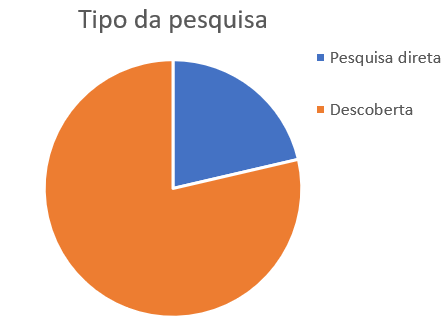
\includegraphics[width=5cm]{imagens/grafico.png}
    \label{figura:qualquernome2}
    \fonteimagem{Fonte: Elaborado pelo autor}
\end{figure}

\begin{figure}[h]
    \caption{Exemplo de imagem B}
    \centering
    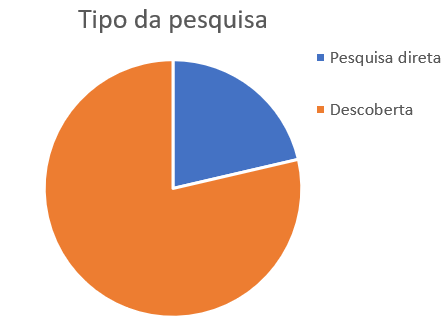
\includegraphics[width=5cm]{imagens/grafico.png}
    \label{figura:qualquernome3}
    \fonteimagem{Fonte: Elaborado pelo autor}
\end{figure}
%
%% ----------------------------------------------------------
%\chapter{Nullam elementum urna vel imperdiet sodales elit ipsum pharetra ligula
%ac pretium ante justo a nulla curabitur tristique arcu eu metus}
%% ----------------------------------------------------------
%\lipsum[55-57]
%
\end{apendicesenv}
%% ---
%
%
%% ----------------------------------------------------------
%% Anexos
%% ----------------------------------------------------------
%
%% ---
%% Inicia os anexos
%% ---
\begin{anexosenv}
%
%% Imprime uma página indicando o início dos anexos
\partanexos
%
%% ---
\chapter{Morbi ultrices rutrum lorem.}
%% ---
\lipsum[30]
%
%% ---
\chapter{Cras non urna sed feugiat cum sociis natoque penatibus et magnis dis parturient montes nascetur ridiculus mus}
%% ---
%
\lipsum[31]
%


\end{anexosenv}
%
%%---------------------------------------------------------------------
%% INDICE REMISSIVO
%%---------------------------------------------------------------------
%
%\phantompart
%
%\printindex

\end{document}
